%%%%%%%%%%%%%%%%%%%%%%%%%%%%%%%%%%%%%%%%%%%%%%%%%%%%%%%%%%%%%%%%%%%%%%%%%%%%%%%%
% Latent Profiles of Academic Achievement Among Rural Students in Peru
% Target journal: Large-Scale Assessments in Education (Springer, Q1)
% Format: Two-column, 12pt
% Reference system: BibLaTeX APA (author-year)
%%%%%%%%%%%%%%%%%%%%%%%%%%%%%%%%%%%%%%%%%%%%%%%%%%%%%%%%%%%%%%%%%%%%%%%%%%%%%%%%

\documentclass[twocolumn,12pt]{article}

%% ── Packages ─────────────────────────────────────────────────────────────────
\usepackage[utf8]{inputenc}
\usepackage[english]{babel}
\usepackage{hyphenat}
\usepackage{graphicx}
\usepackage{amsmath}
\usepackage{amssymb}
\usepackage{url}
\usepackage[margin=2cm]{geometry}
\usepackage{setspace}
\usepackage{fancyhdr}
\setlength{\headheight}{14.5pt}
\usepackage{abstract}
\usepackage{authblk}
\usepackage{multicol}
\usepackage{booktabs}
\usepackage{tabularx}
\usepackage{multirow}
\usepackage{array}
\usepackage{threeparttable}
\usepackage{csquotes}
\usepackage{makecell}   % for \shortstack inside tabular
\usepackage{caption}
\usepackage{svg}
\captionsetup{font=small, labelfont=bf}

%% ── BibLaTeX ─────────────────────────────────────────────────────────────────
\usepackage[
  backend=biber,
  style=apa
]{biblatex}
\addbibresource{references.bib}

%% ── Layout ───────────────────────────────────────────────────────────────────
\setstretch{1.0}
\setlength{\parskip}{3pt}
\setlength{\parindent}{12pt}

\pagestyle{fancy}
\fancyhf{}
\rhead{\thepage}
\lhead{}
\renewcommand{\headrulewidth}{0pt}

\renewcommand{\abstitleskip}{-\parindent}
\renewcommand{\absleftindent}{0pt}
\renewcommand{\absrightindent}{0pt}

%%%%%%%%%%%%%%%%%%%%%%%%%%%%%%%%%%%%%%%%%%%%%%%%%%%%%%%%%%%%%%%%%%%%%%%%%%%%%%%%
%% MANUSCRIPT INFORMATION
%%%%%%%%%%%%%%%%%%%%%%%%%%%%%%%%%%%%%%%%%%%%%%%%%%%%%%%%%%%%%%%%%%%%%%%%%%%%%%%%

\title{\textbf{Latent Profiles of Academic Achievement Among Rural Students
in Peru: An Integrated EFA--IRT--LCA Analysis of PISA Data}}

\author[1]{Kevin Maximiliano Arenas Cancapa}
\author[1]{Eric Raphael Huiza Pereyra%
  \thanks{Corresponding author: \texttt{eric.huiza@pucp.edu.pe}}}

\affil[1]{\small Graduate Program in Computer Science,
  Pontifical Catholic University of Peru, Lima, Peru}

\date{}

%%%%%%%%%%%%%%%%%%%%%%%%%%%%%%%%%%%%%%%%%%%%%%%%%%%%%%%%%%%%%%%%%%%%%%%%%%%%%%%%
\begin{document}
%%%%%%%%%%%%%%%%%%%%%%%%%%%%%%%%%%%%%%%%%%%%%%%%%%%%%%%%%%%%%%%%%%%%%%%%%%%%%%%%

\twocolumn[
\begin{@twocolumnfalse}
\maketitle

%%────────────────────────────────────────────────────────────────────────────
%% ABSTRACT
%%────────────────────────────────────────────────────────────────────────────
\begin{abstract}
\noindent
Academic underperformance in rural Peru represents a persistent structural
challenge, yet the latent factors driving achievement gaps in these contexts
remain poorly understood. This study applies an integrated pipeline of
Exploratory Factor Analysis (EFA), Item Response Theory (IRT), and Latent
Class Analysis (LCA) to PISA 2022 microdata, analysing both the full
Peruvian sample (\(n = 6{,}968\)) and a rural subsample (\(n = 3{,}720\))
defined by community size. EFA across six item blocks identified 35 latent
factors in the rural sample, subsequently refined through IRT screening to
129 high-discrimination items (mean \(a = 1.109\)). LCA revealed four
distinct rural student profiles --- high-performing (20.6\%,
\(M = 446\) pts), medium (25.2\%, \(M = 398\) pts), medium-low (17.2\%,
\(M = 382\) pts), and low-performing (37.0\%, \(M = 355\) pts) --- with
significant between-class differences (\(F = 327.43\), \(p < .001\)).
School management type was the dominant discriminating factor
(\(F = 5{,}430\)): 93.5\% of high-performing rural students attended
private schools, while all remaining classes were composed exclusively of
public-school students. Compared to the national seven-class solution,
rural students required only four latent classes, indicating greater
contextual homogeneity in rural schooling conditions. Post-COVID
pedagogical practices and family cultural capital emerged as secondary
structural determinants specific to rural contexts. These findings provide
empirical evidence for differentiated educational policies targeting rural
subpopulations and demonstrate the analytical utility of integrated
psychometric pipelines for large-scale assessment data.
\end{abstract}

\vspace{0.3cm}
\noindent\textbf{Keywords:} PISA 2022; Latent Class Analysis; Item Response
Theory; Exploratory Factor Analysis; Rural Education; Academic Achievement;
Peru; Educational Inequality; Latent Variables; Educational Data Science
\vspace{0.5cm}
\end{@twocolumnfalse}
]

%%%%%%%%%%%%%%%%%%%%%%%%%%%%%%%%%%%%%%%%%%%%%%%%%%%%%%%%%%%%%%%%%%%%%%%%%%%%%%%%
%% 1. INTRODUCTION
%%%%%%%%%%%%%%%%%%%%%%%%%%%%%%%%%%%%%%%%%%%%%%%%%%%%%%%%%%%%%%%%%%%%%%%%%%%%%%%%

\section{Introduction}

Academic performance in secondary education constitutes a critical indicator
of both educational quality and long-term social development. In Peru, results
from the 2022 cycle of the Programme for International Student Assessment
(PISA) --- conducted by the Organisation for Economic Co-operation and
Development (OECD) --- revealed that only approximately 47\% of students
reached Level~2 or above in Science, 34\% in Mathematics, and 50\% in
Reading, meaning that more than half of assessed students failed to achieve
basic proficiency levels \parencite{oecd2023pisaPeru}.

Rural schools in Peru operate under compounded structural constraints that
may generate patterns of underperformance substantively different from those
observed in urban contexts. This distinction matters analytically: the factors
driving low achievement in rural settings --- including teacher shortages,
limited digital infrastructure, and high socioeconomic vulnerability --- may
not be the same as those operating in urban schools, suggesting that
national-level analyses risk obscuring context-specific mechanisms. Empirical
support for this differentiation comes from the national PISA~2022 results
report, which documents a stark stratification: only 11.0\% of rural students
reached basic proficiency in Mathematics, 21.8\% in Science, and 21.0\% in
Reading, compared to 38.7\%, above 50\%, and above 50\%, respectively, among
urban students \parencite{minedu2024pisareporte}. These gaps motivate the
present study's focus on rural subpopulations as a distinct analytical unit
rather than a subset of the national sample.

Understanding what drives these performance gaps requires moving beyond
observed variables to examine the latent constructs that shape learning
conditions. Contextual factors such as family cultural capital, pedagogical
quality, school governance, and financial literacy operate as unobservable
dimensions that influence student achievement without being directly
measurable in standard assessments. Large-scale datasets such as PISA provide
rich contextual information through student, school, and teacher
questionnaires, but their analytical potential is often underutilised when
studies rely solely on regression approaches or focus on single predictors in
isolation \parencite{rutkowski2010secondary}.

Addressing these unobservable dimensions requires methods specifically
designed for latent variable inference. Recent advances in educational data
science have demonstrated the value of integrating psychometric and machine
learning methods to extract richer insights from large-scale assessment data.
Exploratory Factor Analysis (EFA) enables dimensionality reduction across
high-dimensional questionnaire data; Item Response Theory (IRT) provides
principled item selection based on discrimination and difficulty parameters;
and Latent Class Analysis (LCA) identifies distinct subpopulations with
shared contextual profiles. When applied sequentially, these methods
constitute a principled pipeline for moving from raw survey data to
interpretable student typologies. However, few studies have applied such
integrated pipelines to PISA data in Latin American contexts, and fewer still
have examined rural subpopulations specifically. To our knowledge, no prior
study has applied an integrated EFA--IRT--LCA pipeline to PISA data focusing
on rural students in Peru or any comparable LAC context.

This study addresses that gap by applying an integrated EFA--IRT--LCA
pipeline to PISA~2022 microdata for Peru, with a primary focus on rural
students. The analysis pursues three specific objectives: (i)~to identify
latent dimensions underlying student, school, and family contextual variables
through EFA across multiple questionnaire blocks; (ii)~to refine item
selection using IRT discrimination parameters; and (iii)~to characterise
distinct latent profiles of rural students and examine their association with
academic achievement across mathematics, reading, and science domains.
Additionally, results from the rural subsample are systematically compared
against the full national sample to identify which latent determinants are
context-specific and which reflect broader structural patterns in Peruvian
education.

The remainder of this paper is organised as follows. Section~2 reviews
relevant literature on latent variable methods applied to large-scale
assessments and on educational inequality in Latin America. Section~3
describes the data sources, preprocessing pipeline, and analytical methods.
Section~4 presents results from both the national and rural analyses.
Section~5 discusses findings and their policy implications. Section~6
presents conclusions, limitations, and directions for future research.

%%%%%%%%%%%%%%%%%%%%%%%%%%%%%%%%%%%%%%%%%%%%%%%%%%%%%%%%%%%%%%%%%%%%%%%%%%%%%%%%
%% 2. RELATED WORK
%%%%%%%%%%%%%%%%%%%%%%%%%%%%%%%%%%%%%%%%%%%%%%%%%%%%%%%%%%%%%%%%%%%%%%%%%%%%%%%%

\section{Related Work}

\subsection{Large-Scale Assessments and Educational Inequality in Latin
America}

International large-scale assessments (ILSAs) such as PISA have become
foundational instruments for diagnosing educational inequalities and
informing evidence-based policy across participating countries
\parencite{rutkowski2010secondary}. In the Latin American and Caribbean
(LAC) region, PISA data consistently reveal persistent underperformance
relative to OECD averages, a situation that the COVID-19 pandemic has
considerably worsened. School shutdowns in the region extended for
approximately 270~days on average, representing a disruption equivalent
to 1.42~years of schooling, with the most vulnerable students experiencing
the greatest learning losses \parencite{delprato2025resilience}.

Within Peru specifically, the urban--rural achievement gap constitutes one
of the most structurally entrenched dimensions of educational inequality.
The urban--rural learning gap is largely attributed to differences in school
and family characteristics, with urban areas showing better school resources
and more supportive family environments \parencite{wang2024urbanrural}.
These structural disadvantages are compounded by the public--private school
divide: the self-selection of students into private schools deepens existing
inequalities, and the effectiveness of public and private schools is
additionally affected by their urban or rural location
\parencite{delprato2025schools}. In rural Peru, where private school access
is structurally limited, this stratification mechanism acquires a
particularly pronounced character, as demonstrated by the findings of the
present study.

The COVID-19 pandemic introduced an additional layer of disruption that
differentially affected rural and vulnerable student populations. Evidence
from PISA~2022 indicates that pandemic educational policies produced
differential effects by school type, with policies being more productive in
private than public schools for mathematics, and showing divergent patterns
for students in rural schools under longer periods of closure
\parencite{delprato2025covid}. Teacher retention policies targeting rural
schools have similarly shown limited reach, with bonuses producing modest
effects on learning outcomes that diminish without sustained institutional
support \parencite{castro2022bonuses}. These findings underscore the need
for analyses that disaggregate national-level results by rural context, as
aggregate statistics obscure the unequal distribution of pandemic impacts
across educational subpopulations.

\subsection{Latent Variable Methods in Educational Research}

The identification of unobservable constructs underlying student achievement
has a long tradition in psychometric and educational research. Exploratory
Factor Analysis (EFA) remains a foundational tool for reducing the
dimensionality of large item sets and uncovering latent dimensions in
questionnaire data \parencite{fabrigar1999efa}. Item Response Theory (IRT)
provides a complementary framework by estimating item-level discrimination
and difficulty parameters, enabling principled item selection based on
psychometric quality \parencite{vanderlinden2016irt}. In large-scale
assessments, plausible values --- multiple imputed proficiency estimates
drawn from a conditional distribution to account for measurement uncertainty
--- are the recommended unit of analysis for secondary research using PISA
data \parencite{vondavier2009plausible}.

Latent Class Analysis (LCA) extends the latent variable framework to
person-centred classification, identifying subpopulations of individuals
who share similar response patterns across a set of observed indicators
\parencite{collins2010latent}. The present study implements LCA using
\textcite{morin2025stepmix}'s StepMix, an open-source Python package
implementing pseudo-likelihood estimation for generalised mixture models,
providing flexible one-step estimation with interpretability advantages for
social science applications. The combination of EFA, IRT, and LCA into a
sequential analytical pipeline represents a methodological contribution
with limited precedent in the educational data science literature.

\subsection{Student Profile Analysis Using PISA Data}

Person-centred approaches to PISA data analysis have gained considerable
momentum, driven by recognition that aggregate performance metrics obscure
meaningful heterogeneity in student characteristics and contextual profiles.
Distinct student well-being profiles have been identified using latent
profile analysis on PISA~2018 and 2022~data, with socioeconomic status
consistently associated with less favourable profile membership
\parencite{gorgun2024wellbeing}. Similarly, LCA applied to PISA
questionnaire data has demonstrated that student profiles defined by
motivational and attitudinal variables are systematically associated with
differential academic outcomes across performance domains
\parencite{yi2017lpa}.

Explainable cluster analysis applied to PISA~2022~data has further shown
that student profiles derived from contextual variables can achieve high
interpretability when combined with feature importance methods
\parencite{fernandez2024profiles}. Family cultural capital has been shown to
exert positive direct effects on student cognitive performance across 71
countries in PISA~2022, with effect sizes varying substantially between OECD
and non-OECD countries \parencite{zhang2025capital} --- suggesting that
context-specific analyses targeting rural subsamples are necessary to capture
the heterogeneous operation of these constructs.

\subsection{Machine Learning and Educational Data Mining in Large-Scale
Assessments}

The application of machine learning methods to large-scale assessment data
has expanded substantially over the past decade. Studies combining
statistical and machine learning methods have demonstrated their utility for
identifying predictors of student proficiency in PISA datasets
\parencite{soares2024predictors}. The theoretical grounding for cultural
capital as a determinant of academic achievement draws on
\textcite{bourdieu1986capital}'s foundational framework, which
conceptualises cultural capital as knowledge, skills, and dispositions
transmitted through family socialisation that translate into educational
advantage.

Research on academic resilience in the LAC region using explainable machine
learning and PISA~2022~data has highlighted that studies applying
interpretable methods to global south education systems remain scarce, with
most applications focused on richer country contexts whose realities contrast
sharply with those of developing nations \parencite{delprato2025resilience}.
Collectively, this body of literature establishes three analytical gaps:
(1)~the absence of person-centred latent profile analyses targeting rural
student populations in Peru; (2)~the limited application of integrated
EFA--IRT--LCA pipelines to PISA questionnaire data; and (3)~the
underexploration of how structural factors such as school type and
post-pandemic pedagogical practices shape achievement profiles in rural
educational contexts.

%%%%%%%%%%%%%%%%%%%%%%%%%%%%%%%%%%%%%%%%%%%%%%%%%%%%%%%%%%%%%%%%%%%%%%%%%%%%%%%%
%% 3. METHODOLOGY
%%%%%%%%%%%%%%%%%%%%%%%%%%%%%%%%%%%%%%%%%%%%%%%%%%%%%%%%%%%%%%%%%%%%%%%%%%%%%%%%

\section{Methodology}

\subsection{Data Source and Study Population}

This study uses microdata from the 2022~cycle of PISA, conducted by the
OECD \parencite{oecd2023technical}. For Peru, the assessment included
6,968~students drawn from schools across the national territory. Three
datasets were integrated: the student context questionnaire
(\texttt{STU\_QQQ}), the school questionnaire (\texttt{SCH\_QQQ}), and the
teacher questionnaire (\texttt{TCH\_QQQ}), originally in \texttt{.SAV}
format and converted to \texttt{.CSV}. Records were linked via student
identifier (\texttt{CNTSTUID}) and school identifier (\texttt{CNTSCHID}),
producing a merged dataset of 6,968~observations and 7,147~variables prior
to preprocessing.

\subsubsection{Rural Subsample Definition}

Because PISA~2022 does not provide subnational disaggregation for Peru ---
all records carry the national stratum code --- the rural subsample was
defined using the school-level variable \texttt{SC001Q01TA}, which classifies
the community in which each school is located. Two categories were retained:
\textit{village, hamlet or rural area} (fewer than 3,000 people) and
\textit{small town} (3,000 to approximately 15,000 people). This operational
definition yielded 3,720~rural students (53.4\% of the national sample). The
full national sample was retained as a comparative baseline.

\subsection{Analytical Pipeline Overview}

The analysis follows a sequential four-stage pipeline: (1)~data
preprocessing and variable reduction; (2)~EFA for latent dimension
identification; (3)~IRT calibration for item selection; and (4)~LCA for
student profile identification. Each stage feeds into the next through a
principled reduction of the variable space. The pipeline was applied
independently to both samples.

%% ── FIGURE PLACEHOLDER ───────────────────────────────────────────────────────
%% FIGURE 1 — Methodological pipeline diagram
%% Suggested format: horizontal flow diagram with 5 boxes connected by arrows:
%%   [Raw PISA data] → [Preprocessing] → [EFA: 6 blocks] →
%%   [IRT calibration] → [LCA: profile identification]
%% Below each arrow include the variable counts:
%%   7,147 vars → 573/592 vars → 198 items → 129 items → 4/7 classes
%% Prepare this as a figure and insert it replacing this comment block.
\begin{figure}[ht]
\centering
\includesvg[width=0.9\linewidth]{graphics/pipeline}
\caption{Analytical process from raw PISA microdata to latent student profiles. The numbers indicate the number of variables at each reduction stage for the national and rural samples.}
\label{fig:pipeline}
\end{figure}

%% ─────────────────────────────────────────────────────────────────────────────

\subsection{Data Preprocessing}

The preprocessing stage reduced the initial 7,147-variable dataset through
five sequential filters applied identically to both samples.

\textbf{Step~1 --- Missing data filtering.} Variables with more than 40\%
missing values were eliminated. In PISA, missingness arises structurally
from the modular booklet design, making imputation inappropriate for such
variables \parencite{oecd2023technical}.

\textbf{Step~2 --- Design variable exclusion.} Identifiers, sampling
weights (\texttt{W\_FST}, \texttt{W\_SCH}, \texttt{W\_TCH}), and
OECD-derived composite indices (\texttt{ESCS}, \texttt{HISEI},
\texttt{HOMEPOS}) were removed. Plausible values (\texttt{PV1MATH} --
\texttt{PV10SCIE}) were preserved separately as external performance anchors
for LCA validation \parencite{vondavier2009plausible}.

\textbf{Step~3 --- Free-text exclusion.} Object-type columns with more
than 20\% unique values relative to total rows were removed as
uninformative for factor analysis.

\textbf{Step~4 --- Continuous variable separation.} Numeric columns with
more than 10~unique values were separated from the ordinal item set, as EFA
and IRT require ordinal or categorical inputs.

\textbf{Step~5 --- Near-zero variance elimination.} Variables in which a
single category represented more than 95\% of responses were removed.

Table~\ref{tab:preprocessing} summarises the reduction at each stage.
For variables retained after preprocessing, missing data averaged 7.12\% in
the rural sample; median imputation was applied for EFA and mode imputation
for IRT and LCA.

\begin{table}[htbp]
\centering
\caption{Variable Reduction at Each Preprocessing Stage}
\label{tab:preprocessing}
\scriptsize
\begin{tabular}{@{}lcc@{}}
\toprule
\textbf{Stage} &
  \makecell{\textbf{National}\\(n=6,968)} &
  \makecell{\textbf{Rural}\\(n=3,720)} \\
\midrule
Original variables        & 7,147 & 7,147 \\
After missing $>$40\%     & 1,134 & 1,098 \\
After design var. removal &   893 &   857 \\
After continuous sep.     &   648 &   625 \\
After near-zero variance  & \textbf{592} & \textbf{573} \\
\bottomrule
\end{tabular}
\end{table}

\subsection{Stage 1 --- Exploratory Factor Analysis}

EFA was conducted using the \texttt{factor\_analyzer} Python package,
implementing principal axis factoring with oblimin rotation. Oblique
rotation was preferred because educational constructs --- family support,
school climate, student motivation --- are theoretically and empirically
correlated \parencite{fabrigar1999efa}.

Given the high dimensionality of retained variables, EFA was conducted on
thematically coherent blocks defined by questionnaire origin and variable
prefix, following established practice in large-scale assessment research
\parencite{rutkowski2010secondary}. Six blocks were defined: student items
(\texttt{ST}), three school sub-blocks (\texttt{SC\_a}, \texttt{SC\_b},
\texttt{SC\_c}), financial literacy items (\texttt{FL}), and a residual
block. Prior to extraction, factorability was assessed via KMO and
Bartlett's test; blocks with KMO~$< 0.50$ were excluded. Factors were
retained using the Kaiser criterion (eigenvalue $> 1$) and items retained
at loading $\geq 0.40$.

Table~\ref{tab:efa_blocks} presents adequacy statistics and outcomes for
the rural sample.

\begin{table}[htbp]
\centering
\caption{EFA Results by Questionnaire Block (Rural Sample)}
\label{tab:efa_blocks}
\scriptsize
\begin{tabular}{@{}lccccc@{}}
\toprule
\textbf{Block} & \textbf{Items} & \textbf{KMO} &
  \textbf{Status} & \textbf{Factors} & \makecell{\textbf{Items}\\retained} \\
\midrule
Student (ST)   & 136 & 0.809 & Adequate    & 10 & 47 \\
School A (SC\_a) & 99 & 0.485 & Excluded  & ---  &  0 \\
School B (SC\_b) & 92 & 0.546 & Acceptable & 6  & 34 \\
School C (SC\_c) &109 & 0.557 & Acceptable & 6  & 49 \\
Financial (FL) &  93 & 0.895 & Adequate    &  8 & 51 \\
Other          &  43 & 0.664 & Adequate    &  5 & 17 \\
\midrule
\textbf{Total} & \textbf{572} & & & \textbf{35} & \textbf{198} \\
\bottomrule
\end{tabular}
\end{table}

The exclusion of School Block~A (KMO~$= 0.485$) in the rural sample ---
while it was successfully processed in the national sample
(KMO~$= 0.809$) --- is a substantive finding: governance and evaluation
variables showed insufficient factorial structure in the rural subsample,
likely reflecting the institutional homogeneity of rural schools in Peru,
where most institutions share similar governance constraints imposed by the
national education authority.

%% ── FIGURE PLACEHOLDER ───────────────────────────────────────────────────────
%% FIGURE 2 — Heatmap of EFA factor loadings (rural sample)
%% Suggested format: heatmap with items as rows and factors (F1-F10 for
%% student block) as columns, colour scale from -1 to 1.
%% One heatmap per block, or combined for the two most relevant blocks
%% (Student + School B). This replaces a large factor loading table and is
%% visually more effective in a two-column format.
%% Prepare as figure and insert replacing this comment block.
%% ─────────────────────────────────────────────────────────────────────────────

\subsection{Stage 2 --- Item Response Theory Calibration}

IRT calibration was applied to the 198~EFA-retained items to select those
with adequate psychometric properties. Two models were implemented using the
GIRTH (Georgia Tech Item Response Theory) Python package, which provides
marginal maximum likelihood estimation for unidimensional IRT models:

\begin{itemize}
  \item \textbf{Two-Parameter Logistic (2PL):} for dichotomous items;
        estimates discrimination~($a$) and difficulty~($b$).
  \item \textbf{Graded Response Model (GRM):} for polytomous items
        (3--10 ordered categories); extends 2PL to multiple thresholds.
\end{itemize}

Items were retained if $a \geq 0.50$, a criterion more conservative than
the commonly cited $a \geq 0.35$ \parencite{vanderlinden2016irt}, adopted
to ensure only highly discriminating items entered the LCA.
Table~\ref{tab:irt_results} presents calibration outcomes.

\begin{table}[htbp]
\centering
\caption{IRT Calibration Outcomes (Rural Sample)}
\label{tab:irt_results}
\scriptsize
\begin{tabular}{@{}lcccc@{}}
\toprule
\textbf{Model} & \makecell{\textbf{Items}\\input} &
  \makecell{\textbf{Retained}\\($a \geq 0.50$)} &
  \textbf{Discarded} &
  \makecell{\textbf{Mean}~$a$\\(retained)} \\
\midrule
2PL   &  38 &  21 &  17 & 1.878  \\
GRM   & 160 & 108 &  52 & 0.960  \\
\midrule
\textbf{Total} & \textbf{198} & \textbf{129} & \textbf{69} & \textbf{1.109} \\
\bottomrule
\end{tabular}
\end{table}

%% NOTE FOR REVISION: The "Mean a (retained)" cells for 2PL and GRM
%% separately are left blank. Fill these values from your
%% irt_parametros_retenidos.csv file before submission.

The mean discrimination of retained items in the rural sample (1.109)
exceeded that of the national sample (1.029), indicating that the rural
item set provides sharper differentiation among students along the
measured latent traits.

%% ── FIGURE PLACEHOLDER ───────────────────────────────────────────────────────
%% FIGURE 3 — Discrimination parameter distribution (IRT)
%% Suggested format: side-by-side histogram of discrimination values before
%% and after the a ≥ 0.50 filter, for both rural and national samples.
%% X-axis: discrimination (a); Y-axis: frequency.
%% Vertical dashed line at a = 0.50 threshold.
%% This is more informative than the table alone and shows the filtering
%% effect clearly. Prepare and insert replacing this comment block.
%% ─────────────────────────────────────────────────────────────────────────────

\begin{figure}[ht]
\centering
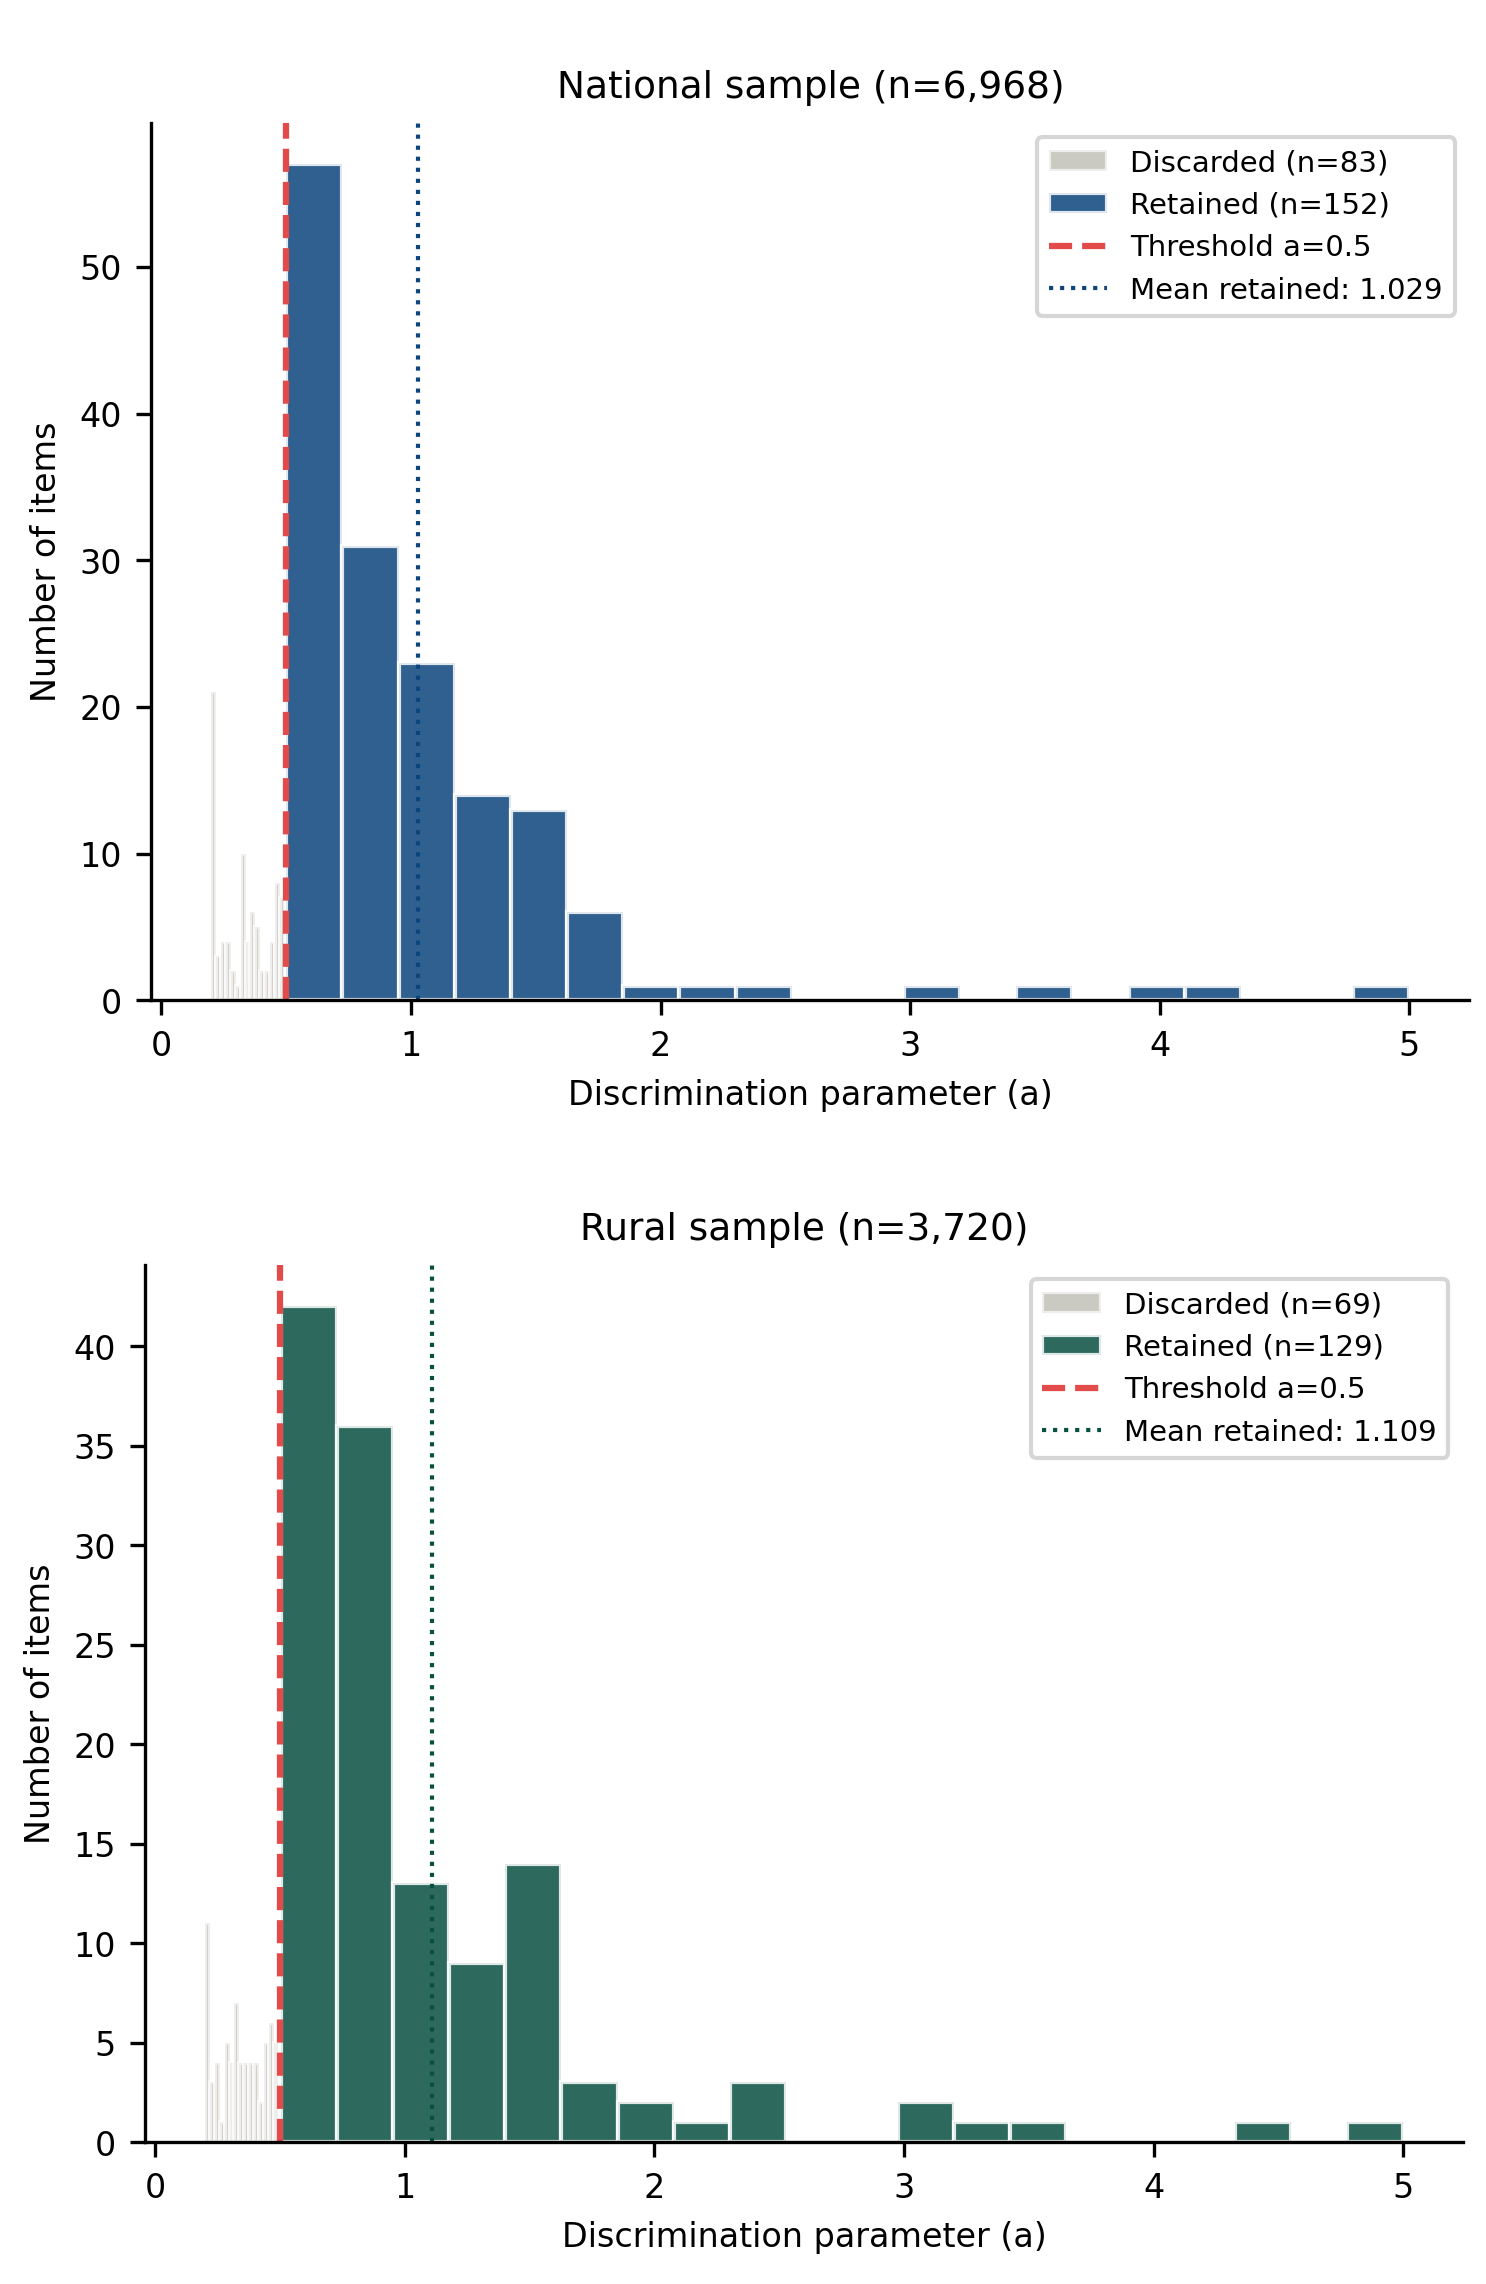
\includegraphics[width=0.9\linewidth]{graphics/fig3_irt_disc_vert.png}
\caption{IRT discrimination parameter distribution — national vs rural sample}
\label{fig:irt_discrimination}
\end{figure}

\subsection{Stage 3 --- Latent Class Analysis}

LCA was conducted on the 129~retained items using StepMix
\parencite{morin2025stepmix} with a categorical measurement model and
one-step estimation (\texttt{measurement="categorical"},
\texttt{n\_steps=1}, \texttt{max\_iter=500}, \texttt{random\_state=42}).

Models with 2--8~classes were estimated and compared using four joint
criteria: (1)~Bayesian Information Criterion (BIC; lower = better fit);
(2)~relative entropy ($\geq 0.80$ indicates adequate classification
certainty); (3)~minimum class size ($\geq 5\%$ of sample,
i.e.\ $\geq 186$~students for rural); and (4)~substantive
interpretability. Class profiles were characterised through a two-layer
strategy: Layer~1 used z-score standardised factor scores to describe
each class along the EFA dimensions; Layer~2 validated classes against
academic performance using the mean of all 30~plausible values across
mathematics, reading, and science as a composite achievement score.
Between-class differences were assessed via one-way ANOVA.

%%%%%%%%%%%%%%%%%%%%%%%%%%%%%%%%%%%%%%%%%%%%%%%%%%%%%%%%%%%%%%%%%%%%%%%%%%%%%%%%
%% 4. RESULTS
%%%%%%%%%%%%%%%%%%%%%%%%%%%%%%%%%%%%%%%%%%%%%%%%%%%%%%%%%%%%%%%%%%%%%%%%%%%%%%%%

\section{Results}

\subsection{Preprocessing and Variable Reduction}

The preprocessing pipeline reduced the original 7,147~variables to
592~ordinal items for the national sample and 573~for the rural subsample
(Table~\ref{tab:preprocessing}). The additional reduction in the rural
sample reflects greater homogeneity in item response distributions, which
caused more variables to fail the near-zero variance criterion.

\subsection{EFA: Latent Factor Structures}

\subsubsection{Rural Sample}

EFA identified 35~latent factors from 198~retained items across five
processable blocks (Table~\ref{tab:efa_blocks}). Table~\ref{tab:efa_factors}
presents the ten student-block factors with their primary items and
interpretive labels.

\begin{table}[htbp]
\centering
\caption{Student-Block EFA Factors --- Rural Sample (10 factors, 47 items)}
\label{tab:efa_factors}
\scriptsize
\begin{tabular}{@{}clp{3.2cm}@{}}
\toprule
\textbf{F} & \textbf{Interpretive label} & \textbf{Primary items} \\
\midrule
1  & Cultural capital \& home resources     & ST254, ST251, ST250 \\
2  & Mathematical learning strategies       & ST268Q07--09 \\
3  & Digital home resources                 & ST250D, ST251D \\
4  & School belonging                       & ST265, ST034 \\
5  & Violence \& school insecurity exposure & ST038, ST266 \\
6  & Participation in maths classes         & ST297 \\
7  & Peer relations \& social belonging     & ST337 \\
8  & Parental educational level             & ST006, ST008 \\
9  & Mathematical self-concept              & ST263Q04, ST263Q06 \\
10 & Extracurricular maths activities       & ST270 \\
\bottomrule
\end{tabular}
\end{table}

%% NOTE FOR REVISION: Replicate a similar condensed table for the
%% school blocks (SC_b 6 factors; SC_c 6 factors) and financial block
%% (8 factors) from your efa_resumen_top_items_por_factor.csv.
%% These can be combined into one table or presented as supplementary material
%% to keep the article within page limits.

\subsubsection{National vs.\ Rural Comparison}

Key structural differences between the national and rural factor solutions
are shown in Table~\ref{tab:efa_comparison}.

\begin{table}[htbp]
\centering
\caption{EFA Structural Comparison: National vs.\ Rural Sample}
\label{tab:efa_comparison}
\scriptsize
\begin{tabular}{@{}p{2.0cm}p{2.3cm}p{2.3cm}@{}}
\toprule
\textbf{Dimension} & \textbf{National} & \textbf{Rural} \\
\midrule
F1 (student)   & Creative activities outside school & Cultural capital \& home resources \\
School Block A & Processed (KMO=0.809) & Excluded (KMO=0.485) \\
Unique factors & Educ.\ expectations; maths anxiety & Peer relations; parental education; extracurricular maths \\
Items retained & 235 & 198 \\
\bottomrule
\end{tabular}
\end{table}

The reordering of the primary student factor --- from creative activities
(national) to cultural capital and home resources (rural) --- indicates
that in rural contexts, material and educational resources in the home
constitute the primary axis of student differentiation, whereas in the
national sample, extracurricular engagement plays that role.

\subsection{IRT: Item Discrimination and Selection}

Of the 198~EFA-retained items, IRT calibration retained 129 for LCA
(65.2\% retention rate). The mean discrimination parameter of retained
items was 1.109 in the rural sample versus 1.029 in the national sample,
confirming that the rural item set captures sharper individual differences.

\subsection{LCA: Latent Class Selection}

Table~\ref{tab:lca_fit} presents model fit indices for 2--8~classes in the
rural sample.

\begin{table}[htbp]
\centering
\caption{LCA Model Fit --- Rural Sample (2--8 Classes)}
\label{tab:lca_fit}
\scriptsize
\begin{tabular}{@{}lcccc@{}}
\toprule
\textbf{Classes} & \textbf{BIC} & \textbf{Entropy} &
  \makecell{\textbf{Min.\ class}\\size (\%)} & \textbf{Viable} \\
\midrule
2 & 844,801 & 0.9997 & ---  & \checkmark \\
3 & 831,527 & 0.9640 & ---  & \checkmark \\
4 & 819,868 & 0.9753 & 17.2\% & \checkmark \\
5 & 815,989 & 0.9783 &  4.3\% & $\times$ \\
6 & 813,541 & 0.9773 &  4.8\% & $\times$ \\
7 & 811,454 & 0.9821 &  4.0\% & $\times$ \\
8 & 809,780 & 0.9819 &  3.8\% & $\times$ \\
\bottomrule
\multicolumn{5}{@{}l@{}}{\footnotesize
  $\times$ = minimum class size $< 5\%$ threshold ($n < 186$).}
\end{tabular}
\end{table}

The 4-class solution was selected as the only model satisfying all four
criteria simultaneously. Models with five or more classes consistently
produced at least one class below the 5\% minimum size threshold
($n < 186$), indicating insufficient statistical power to sustain
finer-grained profiles within the rural population. In the national sample,
the BIC increased at 8~classes (providing a clear inflection point),
supporting a 7-class solution with all classes above 5\% (ANOVA
$F = 397.59$, $p < .001$).

\subsection{LCA: Rural Student Profiles}

Table~\ref{tab:lca_profiles} presents the four rural latent classes with
their academic performance means and school context distribution.

\begin{table}[htbp]
\centering
\caption{Rural Latent Class Profiles: Performance and Context}
\label{tab:lca_profiles}
\scriptsize
\begin{tabular}{@{}lcccc@{}}
\toprule
\textbf{Class} & \makecell{\textbf{Mean PV}\\(pts)} &
  \textbf{SD} & \textbf{n (\%)} &
  \makecell{\textbf{Private}\\school \%} \\
\midrule
1 --- High-performing    & 446.2 & 70.3 & 768 (20.6\%)  & 93.5\% \\
2 --- Medium             & 398.3 & 67.7 & 938 (25.2\%)  &  0.0\% \\
3 --- Medium-low         & 382.2 & 70.3 & 639 (17.2\%)  &  0.0\% \\
4 --- Low-performing     & 354.7 & 59.0 & 1,375 (37.0\%) &  0.0\% \\
\midrule
\multicolumn{5}{@{}l@{}}{\footnotesize
\begin{tabular}[t]{@{}l@{}}
ANOVA: $F = 327.43$, $p < .001$. PV = mean of 30 \\
plausible values (mathematics, reading, science).
\end{tabular}}
\end{tabular}
\end{table}

Class profiles are interpreted along two layers. In Layer~1
(internal characterisation), classes are distinguished by their
standardised factor score profiles (Table~\ref{tab:lca_zscores}).

\begin{table}[htbp]
\centering
\caption{Standardised Factor Scores (z) by Latent Class --- Top Discriminating Dimensions}
\label{tab:lca_zscores}
\scriptsize
\begin{tabular}{@{}lcccc@{}}
\toprule
\textbf{Latent dimension} & \textbf{C1} & \textbf{C2} & \textbf{C3} & \textbf{C4} \\
\midrule
School management type     & $+1.76$ & $-0.48$ & $-0.35$ & $-0.30$ \\
Post-COVID pedagogy        & $-0.40$ & $+0.34$ & $-1.12$ & $+0.52$ \\
Financial literacy (basic) & $+0.41$ & $+0.65$ & $+0.22$ & $-0.66$ \\
Teacher feedback           & $+0.93$ & $-0.37$ & $-0.40$ & $-0.30$ \\
Cultural capital           & $+0.78$ & $+0.23$ & $-0.26$ & $-0.47$ \\
Perceived obstacles        & $+0.80$ & $-0.22$ & $-0.35$ & $-0.25$ \\
Parental education         & $+0.57$ & $+0.18$ & $-0.15$ & $-0.26$ \\
\bottomrule
\multicolumn{5}{@{}l@{}}{\footnotesize
\begin{tabular}[t]{@{}l@{}}
C1=High-performing; C2=Medium; C3=Medium-low; \\ C4=Low-performing.
\end{tabular}}
\end{tabular}
\end{table}

%% ── FIGURE PLACEHOLDER ───────────────────────────────────────────────────────
%% FIGURE 4 — Heatmap of z-score profiles by latent class
%% Suggested format: heatmap with 4 columns (classes) × top 10 latent
%% dimensions as rows. Colour scale: blue (negative) to red (positive).
%% This is the main visual result of the paper and should be publication-quality.
%% Use your figura_perfiles_clases_latentes.png as the base, or regenerate
%% from tabla_perfiles_clases.csv. Insert replacing this comment block.
%% ─────────────────────────────────────────────────────────────────────────────

\begin{figure}[ht]
\centering
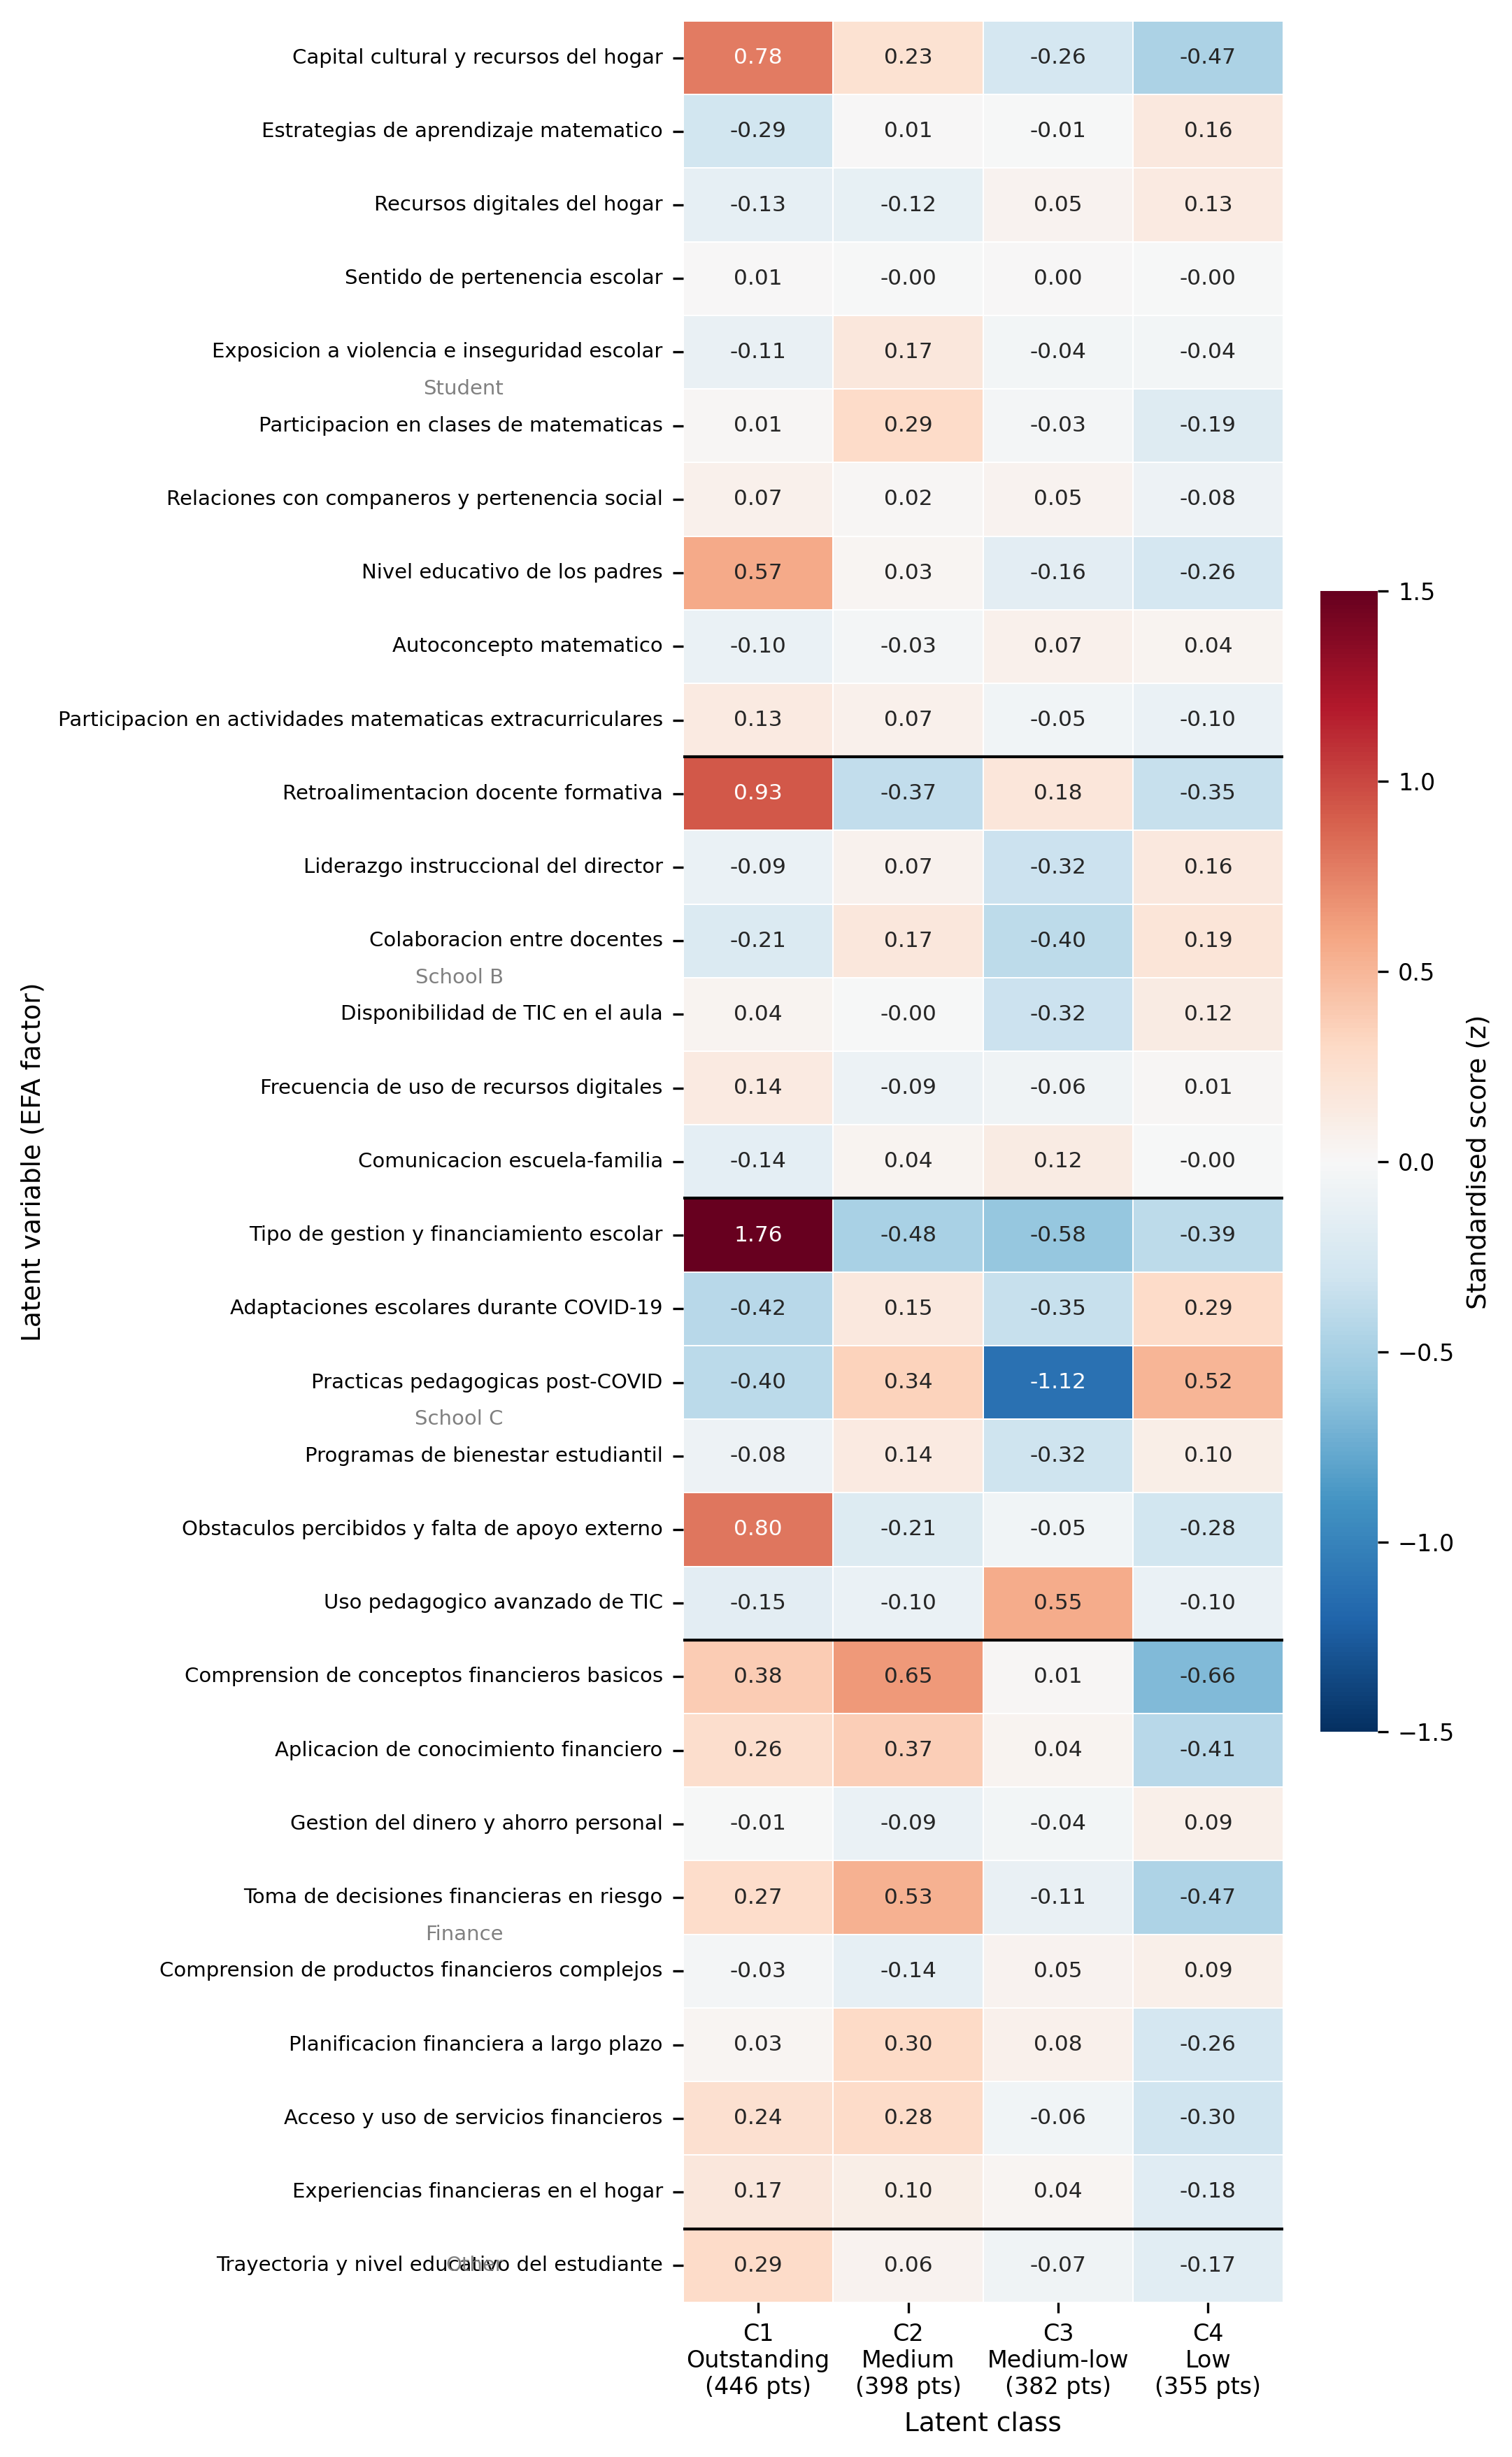
\includegraphics[width=0.9\linewidth]{graphics/fig5_heatmap_perf_clas_rural.png}
\caption{Latent class profiles by EFA-derived latent variables. Rural sample (n=3,720)}
\label{fig:heatmap_perf_class_rural}
\end{figure}

The four profiles are interpreted as follows:

\textbf{Class~1 --- High-achieving students in private rural schools
(20.6\%):} Characterised by private school attendance (93.5\%), strong
teacher feedback ($z = +0.93$), high cultural capital ($z = +0.78$), and
low perceived institutional obstacles ($z = +0.80$). Academic performance
is substantially above the rural mean ($M = 446.2$~pts). Notably, post-COVID
pedagogical adaptation scores are below average ($z = -0.40$), consistent
with private schools having maintained instructional continuity during the
pandemic through pre-existing resources.

\textbf{Class~2 --- Medium performers with financial literacy as protective
capital (25.2\%):} Entirely composed of public school students (100\%).
Distinguished by above-average financial literacy ($z = +0.65$ basic
comprehension; $z = +0.53$ decision-making) despite below-average teacher
feedback ($z = -0.37$) and public school governance ($z = -0.48$). This
profile suggests that practical financial knowledge, likely transmitted
through family economic socialisation in rural contexts, functions as a
compensatory capital that partially offsets institutional deficits.

\textbf{Class~3 --- Medium-low performers with severe post-COVID
pedagogical deficit (17.2\%):} The most rurally concentrated class (58.8\%
in pure rural communities). Characterised by the most extreme post-COVID
pedagogical deficit of any class ($z = -1.12$), low collaborative teaching
($z = -0.40$), and limited technology access ($z = -0.32$). Performance is
$382.2$~pts. This profile indicates that the pandemic's educational impact
was not uniformly distributed among rural students: a distinct, identifiable
subgroup absorbed disproportionately severe pedagogical disruption.

\textbf{Class~4 --- Low-performing students with accumulated structural
disadvantages (37.0\%):} The largest class, representing 37\% of rural
students. Characterised by the lowest financial literacy ($z = -0.66$),
lowest cultural capital ($z = -0.47$), and lowest parental education
($z = -0.26$). Paradoxically, post-COVID pedagogical adaptation is
moderately positive ($z = +0.52$), indicating that schools attempted
adaptation without translating it into improved outcomes. This decoupling
suggests that school-level interventions alone are insufficient to overcome
accumulated family-level disadvantages.

\subsection{National vs.\ Rural Profile Comparison}

The national 7-class solution and rural 4-class solution share the same
dominant discriminating factor (school management type: $F = 2{,}057$
national; $F = 5{,}430$ rural), but the public--private divide is more
extreme in rural contexts: in the national sample, some classes are
compositionally mixed, whereas in the rural sample the high-performing
class is almost entirely private (93.5\%) and all remaining classes are
100\%~public. The second discriminating dimension shifts from creative
extracurricular activities (national, $F = 1{,}105$) to post-COVID
pedagogical practices (rural, $F = 754$), confirming that pandemic-related
factors play a more defining structural role in rural education. The reduced
number of classes (4 vs.\ 7) indicates greater contextual homogeneity in
rural schooling, consistent with the structural constraints of rural
educational systems.

%% ── FIGURE PLACEHOLDER ───────────────────────────────────────────────────────
%% FIGURE 5 — Bar chart: mean academic performance by latent class,
%% national (7 classes) and rural (4 classes) side by side.
%% X-axis: class label; Y-axis: mean plausible value score.
%% Include error bars (±1 SD). Annotate with class size percentages.
%% Prepare from lca_rendimiento_por_clase.csv. Insert replacing this block.
%% ─────────────────────────────────────────────────────────────────────────────

\begin{figure}[ht]
\centering
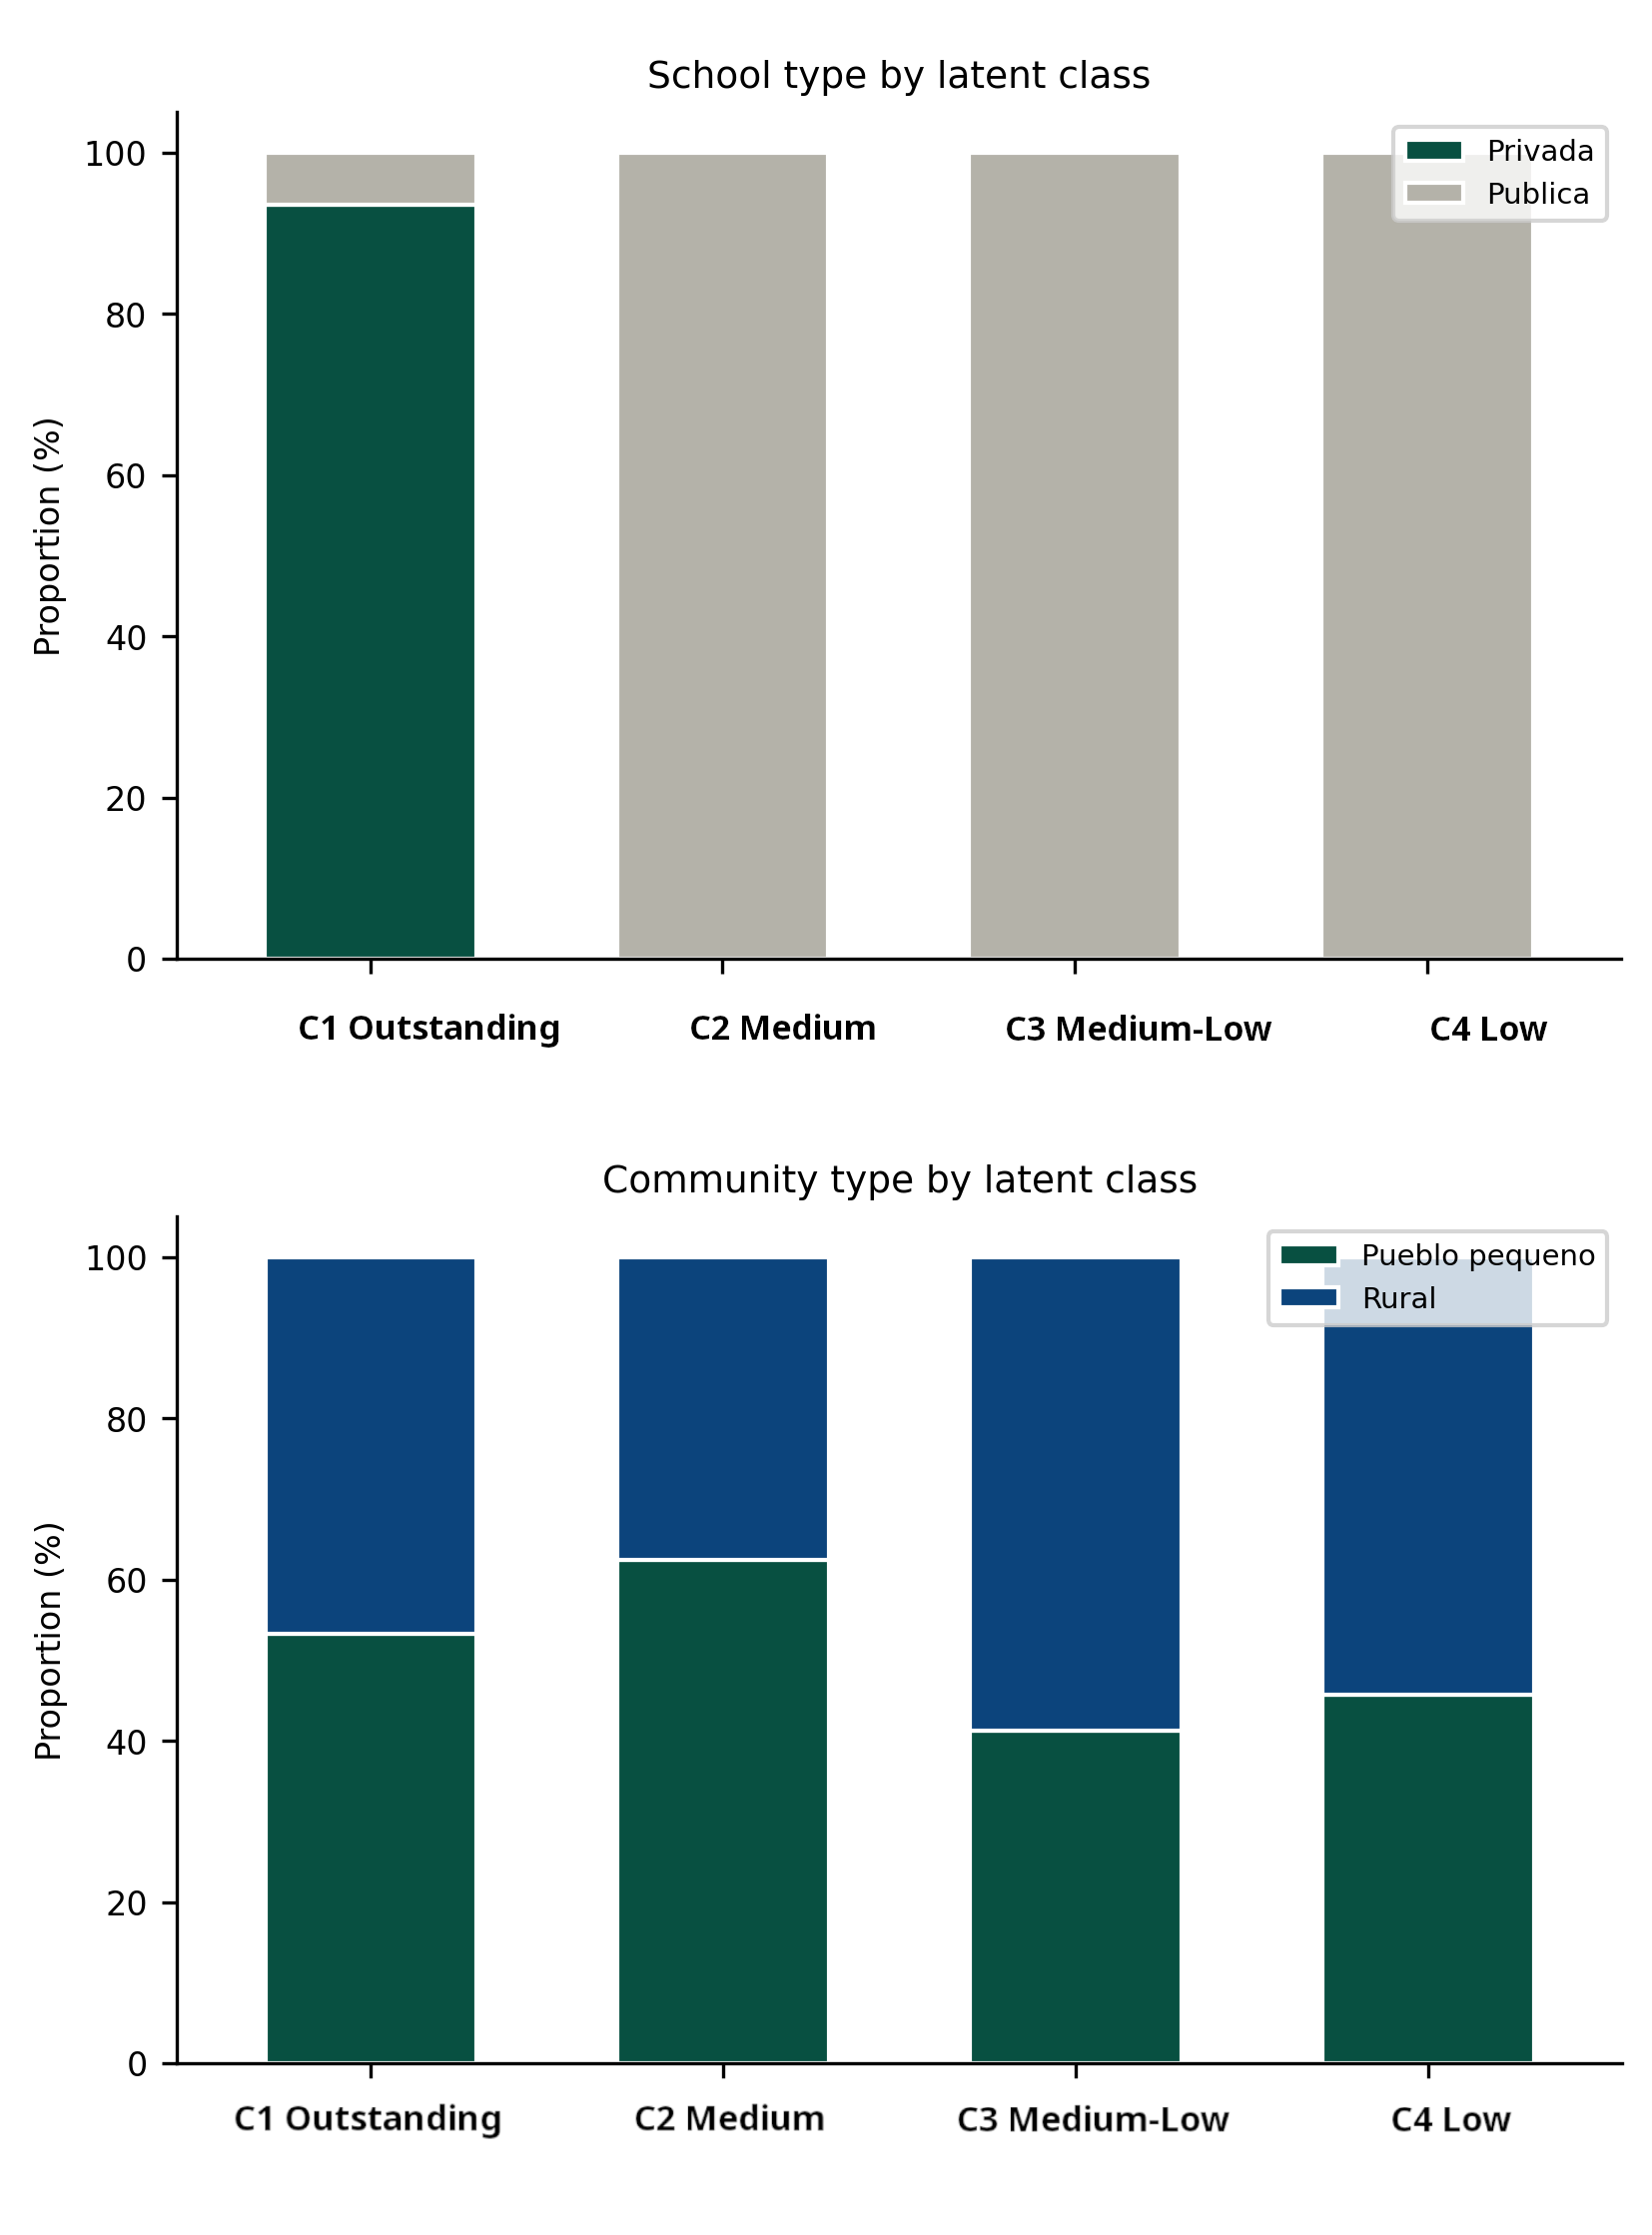
\includegraphics[width=0.9\linewidth]{graphics/fig6_contexto_clases_rural_vert.png}
\caption{Contextual characterisation of latent classes — rural sample (n=3,720)}
\label{fig:context_class_raral}
\end{figure}

%%%%%%%%%%%%%%%%%%%%%%%%%%%%%%%%%%%%%%%%%%%%%%%%%%%%%%%%%%%%%%%%%%%%%%%%%%%%%%%%
%% 5. DISCUSSION
%%%%%%%%%%%%%%%%%%%%%%%%%%%%%%%%%%%%%%%%%%%%%%%%%%%%%%%%%%%%%%%%%%%%%%%%%%%%%%%%

\section{Discussion}

\subsection{The Primacy of School Management Type in Rural Peru}

The most salient finding of this study is the near-absolute segregation
between private and public schooling as the primary determinant of latent
class membership and academic achievement in rural Peru. The dominance of
school management type as a discriminating factor ($F = 5{,}430$) --- with
an effect nearly 2.6~times stronger than in the national sample --- confirms
and extends prior evidence on public--private inequalities in Latin America
\parencite{delprato2025schools}. In rural contexts, where private school
access is structurally limited but not absent, the students who do attend
private institutions constitute a highly advantaged minority whose
performance gap relative to their public-school peers reflects accumulated
advantages in teacher quality, cultural capital, and institutional resources.
This finding has direct implications for policy: strategies targeting rural
education quality must distinguish between the very different institutional
environments in which rural students are educated.

\subsection{Post-COVID Pedagogical Heterogeneity as a Structural Fault Line}

The identification of Class~3 as a distinct profile characterised by severe
post-COVID pedagogical deficit ($z = -1.12$) --- concentrated in the most
rural communities --- provides empirical support for the hypothesis that
pandemic educational disruption was not uniformly distributed within the
rural sector \parencite{delprato2025covid}. While prior research has
documented the general rural disadvantage in pandemic response, the LCA
approach reveals a specific, identifiable subgroup of students who absorbed
disproportionately severe disruption. This subgroup (17.2\% of rural
students) is distinguishable from Class~4 (low performers with accumulated
disadvantages) precisely because their low performance is associated with
pedagogical collapse rather than family-level deprivation, suggesting that
targeted pedagogical recovery programmes could have differential efficacy
for these students compared to the structural interventions required for
Class~4.

\subsection{Financial Literacy as Compensatory Capital in Rural Contexts}

The emergence of financial literacy as a distinguishing dimension between
Classes~2 and~4 --- both entirely composed of public school students ---
suggests a mechanism that has received limited attention in the Latin
American educational research literature. In rural economies where household
financial management is a practical daily necessity, financial knowledge may
function as a form of practical capital that supports cognitive development
independently of formal school quality. This interpretation is consistent
with \textcite{bourdieu1986capital}'s framework of capital forms, extended
here to include practical economic literacy as a context-specific variant of
cultural capital. Future research should examine whether interventions
targeting financial education have spillover effects on academic performance
in rural contexts.

\subsection{Accumulated Disadvantage and the Limits of School Adaptation}

The paradox identified in Class~4 --- where above-average post-COVID school
adaptation ($z = +0.52$) coexists with the lowest academic performance
($M = 355$~pts) and the most severe family-level deficits --- points to a
fundamental limitation of school-centred interventions in contexts of
deep structural disadvantage. This finding is consistent with a growing body
of evidence suggesting that school quality interventions have diminishing
returns in populations facing compound socioeconomic vulnerabilities
\parencite{wang2024urbanrural, castro2022bonuses}. The implication is not
that school adaptation is irrelevant, but that its effects are contingent on
a baseline level of family resources that a significant proportion of rural
Peruvian students (37\%) currently lack.

\subsection{Methodological Contribution}

Beyond its substantive findings, this study demonstrates the feasibility and
analytical value of an integrated EFA--IRT--LCA pipeline applied to PISA
microdata. The sequential logic --- EFA for dimension identification, IRT for
psychometric item selection, LCA for person-centred classification ---
produces interpretable typologies grounded in both statistical rigour and
theoretical coherence. The pipeline's scalability (managing 7,147 initial
variables down to 129 analytically high-quality items) addresses a
persistent challenge in secondary analysis of large-scale assessments, where
the richness of the data often goes underutilised \parencite{rutkowski2010secondary}.

%%%%%%%%%%%%%%%%%%%%%%%%%%%%%%%%%%%%%%%%%%%%%%%%%%%%%%%%%%%%%%%%%%%%%%%%%%%%%%%%
%% 6. CONCLUSIONS, LIMITATIONS, AND FUTURE WORK
%%%%%%%%%%%%%%%%%%%%%%%%%%%%%%%%%%%%%%%%%%%%%%%%%%%%%%%%%%%%%%%%%%%%%%%%%%%%%%%%

\section{Conclusions, Limitations, and Future Work}

\subsection{Conclusions}

This study applied an integrated EFA--IRT--LCA pipeline to PISA~2022
microdata to identify latent profiles of academic achievement among rural
students in Peru. Four distinct profiles were identified, ranging from a
high-performing minority in private schools (20.6\%) to a large vulnerable
majority (37\%) characterised by accumulated family, educational, and
financial disadvantages. The dominant structural determinant was school
management type, whose segregating effect is substantially more pronounced
in rural than in national contexts. Secondary determinants --- post-COVID
pedagogical practices, financial literacy, and cultural capital --- further
differentiate public-school students into meaningfully distinct subgroups
with different intervention needs. Comparison with the national 7-class
solution reveals that rural students present greater contextual homogeneity,
while the same structural factors operate with amplified effect sizes.

Beyond the profile-level findings, the latent factors identified through
EFA constitute the substantive contribution of this study to understanding
what drives academic underperformance in rural Peru. Among the 35~factors
extracted, school management type ($F = 5{,}430$), post-COVID pedagogical
practices ($F = 754$), family cultural capital ($F = 373$), and financial
literacy ($F = 517$) emerged as the dimensions with the greatest
discriminating power across student profiles. These factors are not
abstract statistical constructs --- they correspond to identifiable,
measurable conditions in students' school and family environments.

Critically, the four latent profiles reveal that the rural public-school
population is not homogeneous in its disadvantage. Class~2 students
(\textit{medium performers}, 25.2\%) share the same institutional context
as Class~3 (\textit{medium-low}, 17.2\%) and Class~4 (\textit{low}, 37.0\%)
--- all attend public schools --- yet they are differentiated by distinct
latent dimensions: financial literacy functions as a compensatory resource
in Class~2, post-COVID pedagogical collapse defines Class~3, and accumulated
family-level deficits characterise Class~4. This internal differentiation
within the public-school sector is a finding that aggregate statistics would
not reveal and that has direct implications for how educational interventions
are designed and targeted. From a computational and data science perspective,
this study demonstrates that an integrated psychometric pipeline applied to
large-scale assessment data can produce empirically grounded, actionable
typologies that go substantially beyond what conventional analytical
approaches yield from the same data.

\subsection{Limitations}

Several limitations should be considered when interpreting these findings.
First, PISA~2022 does not provide subnational disaggregation for Peru; the
rural subsample was operationally defined using community size
(\texttt{SC001Q01TA}), which approximates but does not precisely capture
regional characteristics such as those of Andean contexts. Future research
should replicate this methodology using instruments with regional coverage,
such as Peru's ECE national assessment. Second, the modular PISA booklet
design produces structural missing data that cannot be fully resolved through
imputation; the 40\% threshold applied here represents a principled but
necessarily arbitrary cutoff. Third, the LCA solution is data-driven and
the 4-class selection, while supported by multiple criteria, reflects the
statistical power constraints of the rural subsample ($n = 3{,}720$); a
larger rural sample might support more refined profile differentiation.
Fourth, the cross-sectional design of PISA precludes causal inference; the
associations identified between latent profiles and academic outcomes should
be interpreted as descriptive rather than causal. Fifth, School Block~A
variables (governance and evaluation practices) could not be included in the
rural analysis due to insufficient factorial structure (KMO~$= 0.485$),
leaving an important dimension of school functioning uncharacterised in the
rural context.

\subsection{Future Work}

Several directions for future research are indicated by these findings.
Application of the pipeline to Peru's ECE longitudinal data would enable
regional disaggregation and causal inference through panel methods. Extension
to other LAC countries with rural subsamples in PISA~2022 would assess the
generalisability of the identified profiles. The integration of geospatial
analysis to examine the geographic distribution of latent classes within
rural Peru could identify priority intervention areas. Finally, the
development of a confirmatory version of the pipeline (CFA--2PL--LCA) would
allow testing of hypotheses derived from these exploratory findings in
subsequent PISA cycles.

%%%%%%%%%%%%%%%%%%%%%%%%%%%%%%%%%%%%%%%%%%%%%%%%%%%%%%%%%%%%%%%%%%%%%%%%%%%%%%%%
%% REFERENCES
%%%%%%%%%%%%%%%%%%%%%%%%%%%%%%%%%%%%%%%%%%%%%%%%%%%%%%%%%%%%%%%%%%%%%%%%%%%%%%%%

\printbibliography

%%%%%%%%%%%%%%%%%%%%%%%%%%%%%%%%%%%%%%%%%%%%%%%%%%%%%%%%%%%%%%%%%%%%%%%%%%%%%%%%
\end{document}
%%%%%%%%%%%%%%%%%%%%%%%%%%%%%%%%%%%%%%%%%%%%%%%%%%%%%%%%%%%%%%%%%%%%%%%%%%%%%%%%
